% This is "www2010-sample.tex" copied from "www2005-sample.tex" V1.2 January 26 2004
% This file should be compiled with V1.4 of "www2010-submission.class"
%
% This example file demonstrates the use of the 'www2010-submission.cls'
% V1.4 LaTeX2e document class file. It is for those submitting
% articles to the WWW'04 Conference WHO DO NOT WISH TO
% STRICTLY ADHERE TO THE SIGS (PUBS-BOARD-ENDORSED) STYLE.
% The 'www2010-submission.cls' file will produce a similar-looking,
% albeit, 'tighter' paper resulting in, invariably, fewer pages.
%
% ----------------------------------------------------------------------------------------------------------------
% This .tex file (and associated .cls V1.4) produces:
%       1) NO Permission Statement
%       2) WWW'04-specific conference (location) information
%       3) The Copyright Line with ACM data
%       4) NO page numbers
%
% ---------------------------------------------------------------------------------------------------------------
% This .tex source is an example which *does* use
% the .bib file (from which the .bbl file % is produced).
% REMEMBER HOWEVER: After having produced the .bbl file,
% and prior to final submission, you *NEED* to 'insert'
% your .bbl file into your source .tex file so as to provide
% ONE 'self-contained' source file.
%
% ================= IF YOU HAVE QUESTIONS =======================
% Questions regarding the SIGS styles, SIGS policies and
% procedures, Conferences etc. should be sent to
% Julie Goetz (goetz@acm.org) or Adrienne Griscti (griscti@acm.org)
%
% Technical questions only to
% Gerald Murray (murray@acm.org)
% ===============================================================
%
% For tracking purposes - this is V1.2 - January 26 2004
\documentclass{www2010-submission}

\begin{document}
%
\title{Search the Web Using GUI Screenshots}
%\subtitle{[Extended Abstract]
%\titlenote{A full version of this paper is available as
%\textit{Author's Guide to Preparing ACM SIG Proceedings Using
%\LaTeX$2_\epsilon$\ and BibTeX} at
%\texttt{www.acm.org/eaddress.htm}}}
%
% You need the command \numberofauthors to handle the "boxing"
% and alignment of the authors under the title, and to add
% a section for authors number 4 through n.
%
% Up to the first three authors are aligned under the title;
% use the \alignauthor commands below to handle those names
% and affiliations. Add names, affiliations, addresses for
% additional authors as the argument to \additionalauthors;
% these will be set for you without further effort on your
% part as the last section in the body of your article BEFORE
% References or any Appendices.

\numberofauthors{2}
%
% Put no more than the first THREE authors in the \author command

% NOTE: All authors should be on the first page. For instructions
% for more than 3 authors, see:
% http://www.acm.org/sigs/pubs/proceed/sigfaq.htm#a18





\author{
%
% The command \alignauthor (no curly braces needed) should
% precede each author name, affiliation/snail-mail address and
% e-mail address. Additionally, tag each line of
% affiliation/address with \affaddr, and tag the
%% e-mail address with \email.
\alignauthor Tom Yeh, Brandyn White, Larry Davis\\
       \affaddr{University of Maryland}\\
       \affaddr{College Park, MD, USA}\\
       \email{\{tomyeh, bwhite, lsd\}@umd.edu}
%\alignauthor Brandyn White\\
%       \affaddr{Institute for Clarity in Documentation}\\
%       \affaddr{P.O. Box 1212}\\
%       \affaddr{Dublin, Ohio 43017-6221}\\
%       \email{webmaster@marysville-ohio.com}
%\alignauthor Larry S. Davis\\
%       \affaddr{Institute for Clarity in Documentation}\\
%       \affaddr{P.O. Box 1212}\\
%       \affaddr{Dublin, Ohio 43017-6221}\\
%       \email{webmaster@marysville-ohio.com}
\alignauthor Boris Katz\\
       \affaddr{CSAIL}\\
       \affaddr{Cambridge, MA, USA}\\
       \email{boris@mit.edu}
}
\additionalauthors{Additional authors: John Smith (The Th{\o}rv\"{a}ld Group,
email: {\texttt{jsmith@affiliation.org}}) and Julius P.~Kumquat
(The Kumquat Consortium, email: {\texttt{jpkumquat@consortium.net}}).}
\date{30 July 1999}
%\begin{figure*}[t]
%
\includegraphics[width=2\columnwidth]{authors.png}
%\end{figure*}
\maketitle

\begin{abstract}
This paper provides a sample of a LaTeX document which conforms,
somewhat loosely, to the formatting guidelines for
ACM SIG Proceedings. It is an {\em alternate} style which produces
a {\em tighter-looking} paper and was designed in response to
concerns expressed, by authors, over page-budgets.
It complements the document \textit{Author's (Alternate) Guide to
Preparing ACM SIG Proceedings Using \LaTeX$2_\epsilon$\ and Bib\TeX}.
This source file has been written with the intention of being
compiled under \LaTeX$2_\epsilon$\ and BibTeX.
The developers have tried to include every imaginable sort
of ``bells and whistles", such as a subtitle, footnotes on
title, subtitle and authors, as well as in the text, and
every optional component (e.g. Acknowledgments, Additional
Authors, Appendices), not to mention examples of
equations, theorems, tables and figures.
To make best use of this sample document, run it through \LaTeX\
and BibTeX, and compare this source code with the printed
output produced by the dvi file. A compiled PDF version
is available on the web page to help you with the
`look and feel'.
\end{abstract}

% A category with only the three required fields
\category{H.4.m}{Information Systems}{Miscellaneous}
\category{D.2}{Software}{Software Engineering}
%A category including the fourth, optional field follows...
\category{D.2.8}{Software Engineering}{Metrics}[complexity measures,
performance measures]

\terms{Image search}

\keywords{Image search}

\section{Introduction}

There are a lot of resources on the Web about software
applications. Users can learn from these resources teach how to
perform a wide variety of tasks such as setting up a home network,
backing up files, or changing the speed of the mouse cursor. These
resources are often created and made available online by software
developers themselves who wish to maintain an online version of
the documentation apart from the built-in one in order to keep the
content always up-to-date (e.g., support.microsoft.com). These
resources are also created by unofficial, third-party experts, for
example, by sites offering tutorials and tips on various software
applications (e.g., osxfaq.com), by general-purpose \emph{how-to}
sites (e.g., eHow.com) featuring software tutorials as one of the
topics, and by computer book publishers who wish to make their
books accessible online via subscription (e.g.,
safaribooksonline.com). Even more resources can be found in
user-generated contents, for example, in blogs where bloggers
share their experiences and tips using the software application,
in discussion boards where people can discuss and learn from each
other about software, and in QA communities such as Yahoo Answers
where members can raise question and get answers back from other
members.

However, for some users, searching this valuable resource
effectively can be challenging. For example, suppose a user opens
up the network properties dialog window and wishes to find out how
to change the IP address. To use a search engine, this user may
first type ``change IP address'' to describe the task he wishes to
learn. He may soon realize it is also necessary to indicate which
dialog window he wishes to perform the task with. To do so, he may
enter additional search terms to describe the operating system,
the title of the dialog window, and any other information needed
to identify the dialog window. Not only is it \textbf{cumbersome
to enter many keywords} but also these keywords are \textbf{prone
to ambiguity} since it is hard distinguish the keywords describing
the program from those describing the task. Moreover, as the user
browses the links in the result, the user may find it
\textbf{difficult to judge relevancy} based only on the summary
text. The emphasis on second language education and the
availability of free and powerful machine translation technology
(e.g., Google Translate) have enabled many Web users to perform
bilingual search in order to access more information beyond the
confine of their native languages. However, technical articles are
often \textbf{inaccessible by bilingual search}. For example, a
Chinese-speaking person fluent in English may be able to retrieve
useful articles on dogs in both languages using the English or
Chinese word for \emph{dog} as the search term. But when it comes
to technical terms such as \emph{system preferences}, the same
person may be confined to only Chinese articles since it is not
obvious how to translate these terms into English.

separating entities and topics

%Users often rely on the names displayed on the interface to
%describe keywords. Many non-English speaking users use localized
%software in their native language. They can read and understand
%English well or use a machine translator such as Babel to help
%them understand. While translating common terms is easy,
%translating technical interface names is hard, making the
%English-language resources inaccessible to these international
%users.


(The ranking in this example has been artificially adjusted in
order to illustrate a rich variety of results.)

\begin{figure*}
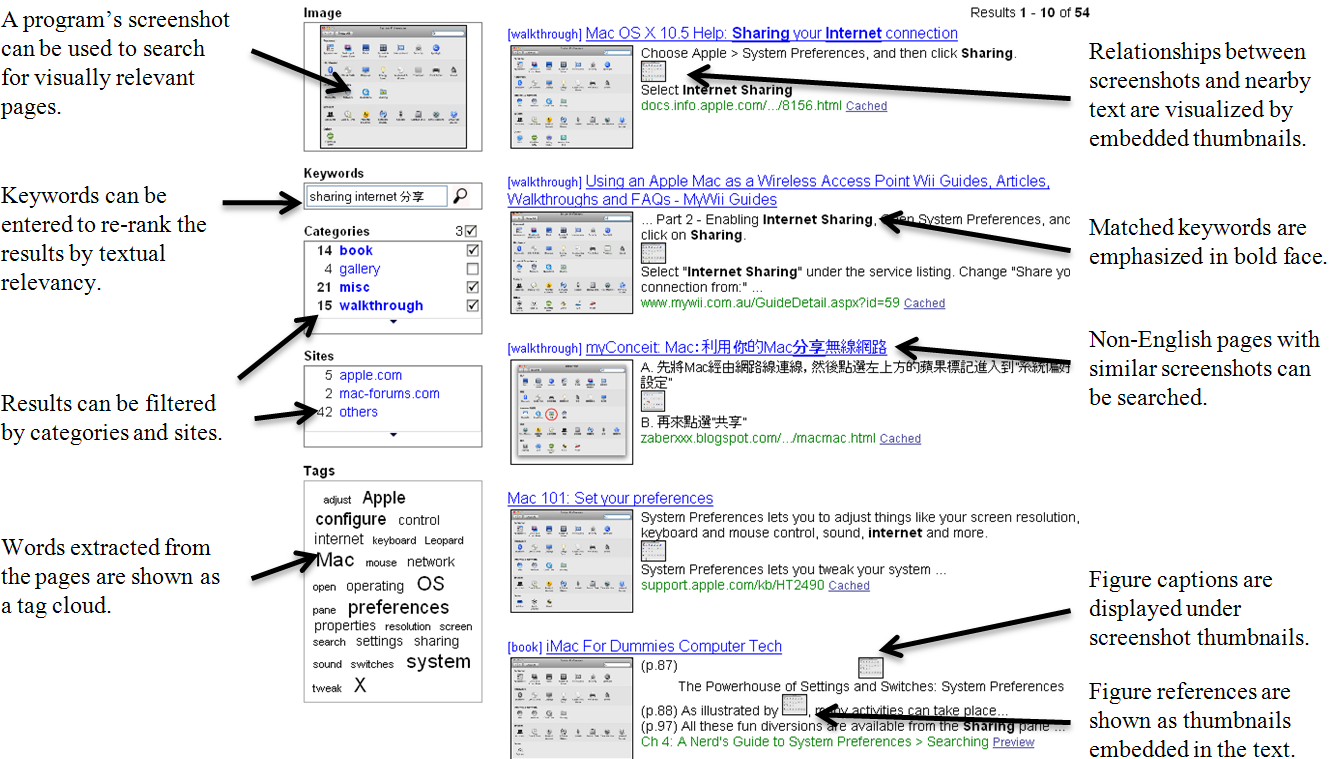
\includegraphics[width=2\columnwidth]{figure/main_result.png}
\end{figure*}

%One possibility is to choose the words at the title of the window
%as keywords. The user also needs to specify what a
%
%* Need to type many keywords. Most cases copy and paste is not supported.
%* Ambiguity: how to do X with Y? But keywords are all the same.
%* Hard to judge the relevancy.
%* Sometimes in a long document with multiple steps, it's unclear
%where in the document is relevant to the current screen.
%* can not search cross langauge (bi-lingual who may be familiar
%with the terms in one language but can read the explanation in two
%languages equally well)

C: Use multi-modal search
    Brief system demo
        walk through a search scenario
        showoff the scale
    Explain how each limitation is overcome
    List of contributions
        Propose a new large-scale search system
        Evaluate it
    Road map

\section{Related Work}

There has been a growing research interests in the indexing,
searching, and organzing images on the web. Many researchers shared
their results in the recent WWW conferences.  Many classic IR problems
have been revisited in a new context of images The Spam problem.
Mehta et al \cite{Mehta} tackled spam that are images using visual
features and near duplicate detection.  The result
diversfication. Kennedy and Naaman \cite{Kennedy} focused on how to
generate a divserse and represenative search results fo landmark
images. van Leuken et al \cite{vanLeuken} also dealt with diverse
image search results based on visual clustering. Some dealt with
organizing photos. The ranking problem. Jing and Baluja \cite{Jing}
tried to improe the ranking of product images using PageRank.  The
relevancy judgement problem. Arase et al \cite{Arase} proposed a
game-based approach to college human assigned relevancy of landmark
images. Li et al \cite{Li} focused on imporving the relevance
judgement of web search results with image excerpts, identifying the
dominant image in a page and displyaing it in the excerpt.  Authority
identification problem. Lempel and Soffer \cite{Lempel} built a image
retrieval system; by analysing link structure, they determine whether
an image is coming from an authoritive source without using any visual
information.  Crandall et al \cite{Crandall} proposed a technique of
organizing a large dataset of geotagged photos using visual, textual,
and temporal features. In relation to these works, ours depend on
state-of-the-art visual analsis techniques to index and search
images. But unlike these works, rather than the end, searching images
is a mean to the goal of finding useful information.

Growing interests in cross language. Tanaka-Ishii and Nakagawa
\cite{Tanaka-Ishii} built a usage consultation tool for language
learner to engage in multi-lingual search to find the usage of any
string of words. Scholl et al \cite{Scholl} explored ways to recognize
web genres in a language independent manner based on structure of HTML
markup. Ni et al \cite{Ni} seek ways to analyze and organize Web
information written in different languages, mininig multilingual
topics from Wikipedia. In relation to these works, the current work
offers another interesting possiblity---searching based on the
univesal visual language of screenshots.

There is also focus on helping comptuer users. Medhi et al \cite{Medhi}
studied the optimal way of presenting audio-visual know-how knowledge to
novice computer users.

Several works have been presented to enablge users to search in more
than one modalities. Narayan et al \cite{Narayan} studied multi-modal
interfaces for mobile devices for accessing web information through a 
personalized dialog based interaction basedon speech and text. 
Dowman et al \cite{Dowman} studied the problem of indexing and
searching radio and televiton news using speech recognition transcript and text
and meta data of the web pages containg related news. Our multi-modal
search is to use image and keywords with faceted search capabilties.

Amazon mechanical turk. In several components of the current work, we
applied AMT for bot training and testing.  Recently, many works have
used AMT for labeling training images and for evaluating
systems. Kittur et al \cite{Kittur} experimented the capabiliy of AMT
to perform user stuides for collecting ratings of Wikipedia articles
that match expert judgements.  In IR, Liu et al \cite{Liu} used AMT
successfully to evaluated the system for predicting seeker
satisfcation in online QA communicties, and offer researchers without
lots of resources like commercial entities to conduct large-scale
experiments.  They identified advantages, low cost and covers a wide
demographics than lab-based studies.  In comptuer vision, XXX used AMT
to evaluate their results. However, as identified by \cite{Liu}, there
are certain risks associted with this method.  risks of getting
dishonest answers unless tasks are forumlated in such a way that the
optimal strategy for workers is to perform the task in the honest
manner. This has been a focus of some researchers in the IR
community. For example, Kazai et al \cite{Kazai} proposed a social
game based method for quality control of relevance assessment. In
all of our applications of AMT, we built in validation 
mechansism to control quality.

\section{Building the database}

\subsection{Collecting images}

%With lots of resources like a commercial search companies, it is
%possible to crawl the web and collect a large number of
%screenshots. As an academic research project, we are limited by
%resource. Yet, we still manage to build a research prototype
%database at a non-trivial scale of 100,000 images. These images
%came from three sources.

We used three methods to collect screenshot images to populate our
database. Currently, our prototype system contains a total of
150,000 images in its index.

First, we submitted computer-related keywords to Bing Image Search
to collect screenshot images of interactive programs. To increase
the likelihood of obtaining the desired images, we sampled
keywords from title bars of the dialog windows of various computer
programs. Some examples of these keywords are properties,
preferences, option, settings, wizard, custom, installation,
network, sound, keyboard ....etc. We turned on the filter feature
to keep only illustration and graphics, rejecting obviously
non-screenshot images such as images of faces and natural scenes.
Using this method, we collected a total of 100,000 images, about
80\% of them are screenshots of computer programs.

Second, we used TinEye, a reverse image search engine that can
take an image as the query and return a list of URLs to nearly
identical copies of the image found on the Web for copyright
infringement. We manually captured screenshot images of more than
300 interactive windows of popular programs across three of the
most popular OS platforms (XP, Vita, and Mac OS). These images
were submitted to TinEye to obtain about 5,000 images. Since the
visual similarity matching performed by TinEye is very precise,
all of these images are screenshot images.

Third, we collected a library of 102 electronic books on popular
software programs. We extracted all the image figures embedded in
the electronic file (i.e., Pdf documents). About x\% of these
figures are screenshots. This method gave us about 50,000 images.

Each method has its own pros and cons. While Bing Image Search
provides the best variety of images, many of them are not visually
relevant to any program at all. TinEye is able to provide visually
relevant images. But these images are ranked only by visual
relevancy; the page containing the highest ranked image may not
necessarily contain any useful information. Computer books are
professionally edited and thus containing the highest quality
text. But they cover a relatively limited range of applications
and their contents are less up-to-date compared to the Web. By
using all these methods, we hope to create a rich repository of
technical information that is both visually and textually relevant
to and accessible by general computer users.


%Since we were constrained by the limit of 1000 images imposed by
%Bing's API, we needed to use different combinations of keywords in
%order to explore different parts of the index.
%
%We submitted different combinations of computer-related keywords
%as search terms to Bing Image Search. We retrieved the first 1,000
%results and downloaded the images as well as the web pages
%containing those images.

%While in most image search applications false positive in search
%results may be a curse, it is a blessing for data collection
%purpose. For example, using system preferences as search terms,
%while more than half of images are indeed screenshots of the
%system preferences window, many images are of other interactive
%windows that happen to be on pages that contain either the keyword
%system or the keyword preference. Nevertheless, these screen
%images are useful for users who happen to wish to query the system
%about those interactive windows.

%The API has restriction to only the top 1000 results. To increase
%the likelihood of having a screenshot image, we use the filter
%function to restrict to only illustration and graphics (namely,
%ignoring natural photographs). In most cases, about 80\% are left.
%In theory it is possible to greatly expand the database if we have
%inside access to the index of the commercial search engines. We
%obtained a total about 50,000 images.


\subsection{Indexing images}
Challenges are:
1. There are a lot of screenshot images.
2. There are different sizes.
3. Some of them are cropped.
4. Some of them are superimposed on a larger image.
5. Some of the components may be rearranged. For example,
in system prefrences, the icons may have shifted.

Exaplin how using hamming embedding and related techniques can
help us deal with each of these challenges.

\subsection{Extracting Text}

After collecting and indexing a large number of screenshots, we need
to extract relevant text from the source articles of these
screenshots. The objective of text extraction is to identify snippets
in an article that can highlight and/or give hints about the kinds of
knowledge users can expect to obtain if they read the article. For
example, for an article containing a screenshot of the network
configuration program, a good snippet would be ``set IP address'' or
``enable wireless network'' since it clearly indicates to users the
article is likely to explain how to perform these tasks. On the other
hand, a snippet such as ``network configuration'' that describes the
screenshot's content is less useful to users since they already see
the content in the screenshot and learn nothing new from reading the
content again in the snippet. Note that this is in sharp contrast with
typical image search engines that actually favor snippets describing
image contents in order to index and search images. Below we list N
types of informative snippets we extract for the purpose of our 
search application:

\begin{description}

\item[Title] We extract the text in the Title tag from the HTML
  header. For book, we simply use its title.

\item[Heading] Compard to title, heading provides more specific
  information regarding the topic of an article containing a
  screenshot. Heading is especially useful when there are multiple
  screenshots contained in the same article. For web articles, we
  extract the heading tag (e.g., h1,h2) cloeset to and proceeding each
  screenshot. For book articles, we extract the chapter and section
  headings from the outline metadata stored in the PDF file whenever
  such metadata is available.

\item[Alt Text] An image's ALT tag provides information redundancy in
  case when the image fails to be displayed. The text attrbute of an
  ALT tag is often a useful feature for a keyword-based image search
  engine to index and search images. Based on our observation, the Alt
  text of the screenshot of a program (e.g., System Preferences) tends
  to be the title of the program (e.g., Alt=``system preferences'').
  Thus, such text may not provide any additional information other
  than what the users can already read directly on the computer
  screen. Yet, we expect Alt text can still be helpful in
  strengthening users' confidence in a search result, by checking
  whether both the program's screenshot and title appear in the
  result's excerpt.

\item[Caption] Many screenshot images are accompanied by caption text
  to briefly describe the idea meant to be illustrated by the images.
  Especially in books, almost all the figures, whether or not they are
  screenshots, contain captions that can reliably extracted by looking
  for string patterns that begin with the word Figure.  Even in the
  articles on the web, captions can sometimes be found below or above
  images. These captions are harder to detect because often they are
  not explicitly labeled by the word Figure. Thus, we identify
  potential caption text based on two simple heuristics: (1) is it
  immediately above or below the image and (2) does it have a
  different style from those of surrounding paragraphs.

\item[References] Sometimes references to images can be found in
  sentences relatively away from the images. Some references are based
  on explicit labels, such as the phrase \emph{as shown in Figure
    X}. Some references are based on layout relationships, such as
  such as the phrase \emph{see below}. Sentences containing such
  references are likely to relevant to the images they refer
  to. Presented in the excerpt, these sentences may indicate the types
  of knowledge users can expect to learn if they read the whole
  article. To resolve a label-based reference, we look for the image
  whose caption contains the matching label. For web articles, the
  image is always on the same page, whereas in book articles, the
  referred image can appear a few pages away due to formatting
  limitations. To resolve a layout-based reference, we scan in the
  direction indicated in the reference (e.g., scan backward for see
  below) until an image is found. After resolving the reference, a
  link between the referred image and the referring sentence is
  established. Whenever an image is retrieved, sentences referring to
  it can also be retrieved to be included in the excerpt.

\item[Action Phrases] Since one of the anticipated uses of our systems
  is to learn how to perform interactive actions using a particular
  program, phrases containing certain action keywords can potentially
  be useful. For examples, phrases containing keywords such as
  configure, click, and open, may indicate to the users that the
  article are likely to explain what can be configured, what should be
  clicked, and what must be opened, using the program. Thus, we
  compile a list of common action keywords and extract action phrases
  from each images' surrounding text.

\item[Nearby Text] If none of the above useful excerpt phrases can be
  extracted, we simply extract nearby sentences around the image and
  use it as the exceprt.

%% \item[Figure OCR] Useful text are those the user does not already
%% know. Text that can also be found in the figure is not as useful.
%% Thus, we apply OCR on each figure to determine what text is
%% already embedded in each figure. While these OCR text might not be
%% that useful to the users, since they can already read them, such
%% text can be useful for filtering out sentences that are simply
%% repeat of what is in the figure and thus less useful to the users.

\end{description}

\subsection{Classifying articles into categories}

In addition to extracting useful text from articles, we can also
classify them into distinct categories based on their origins,
structures, and contents.  In the current work, we consider four
categories: book, walkthrough, gallery, and general. The book category
consists of those articles extracted from pdf books. The walkthrough
category includes articles giving step-by-step instructions on how to
perform certain computing tasks such as backuping files and changing
display resolution. Figure \ref{fig:example_walkthrough} shows some
examples of walkthrough articles. These walkthrough articles tend to
possess three features that can help us identify them. First, they
tend to contain an ordered or unordered list of instructions in short
sentences interpersed with screenshot illustrations.  Second, these
sentences tend to begin with common interactive action verbs such as
click, enter, type, and open. Third, walkthrough articles tend to
include certain indicative terms such as the very word walkthrough,
step, and guide. The gallery category consists of articles with many
images but relative small amount of text. The general category covers
all the unclassified article. Table \ref{} summarizes the 
distribution of articles over the categories. 

\begin{figure}
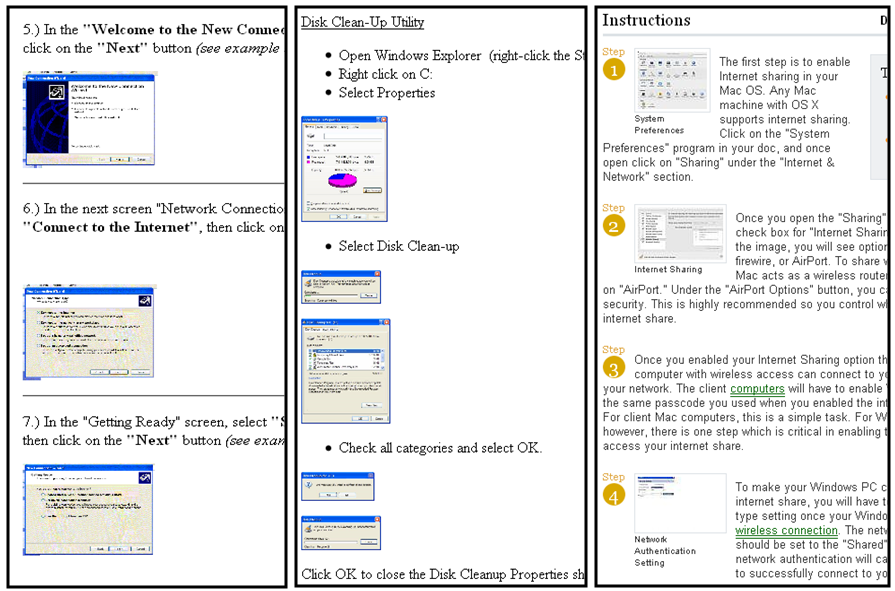
\includegraphics[width=1\columnwidth]{figure/walkthrough_examples.png}
\caption{Examples of articles providing step-by-step walkthroughs.}
\label{fig:example_walkthrough}
\end{figure}

About 28.7\% of articles are classified as walkthrough, while a
small number of articles are classified as galleries (about 2.8\%).

\begin{table}
\centering \caption{Number of images in each category.} \label{}

\begin{tabular}{|c|c|c|c|c|}
\hline
  % after \\: \hline or \cline{col1-col2} \cline{col3-col4} ...
      & General & Walkthrough & Gallery & Book \\
\hline
Total & 34,509 & 30,449 & 2,943 & 55,244\\
 \hline
(\%)  & 32.7 & 28.7 & 2.8 & 35.6 \\
\hline
\end{tabular}
\end{table}

\subsection{Statistics}

What are the websites hosting the most number of screenshots?

What are the types of websites hosting useful screenshots?


\section{Searching the database}

\subsection{Specifying queries}

Sikuli Search supports mixed-modality queries in order to optimize
the effectiveness in searching technical articles about
interactive programs. A typical query to Sikuli Search consists of
a screenshot of a program and, optionally, a set of keywords to
specify what aspects of the program the retrieved articles are
supposed to cover.

Screenshot queries can be specified in two ways. First, users can
run a cross-platform, Java-based client interface we developed to
capture the screenshot of a selected window or an arbitrary screen
region. The client interface will submit the screenshot as the
image query to Sikuli Search and display the search results in the
default web browser. Alternatively, users can use any existing
image capture utilities such as the snipping tool on Windows Vista
or the Command-Shift+4 hotkey on Mac OS to capture screenshots.
Users can use a Web interface to submit the screenshots to Sikuli
Search and view the results directly.

Keywords queries are optional and can be specified in three ways.
They can be entered together with the screenshot queries on both
the client and Web interfaces. Also, as the users are browsing the
results, they can enter keywords to filter and/or refine the
results.

\subsection{Finding similar images}


\subsection{Ranking pages}

Since our search application involves both images (i.e., screenshots)
and text, we can not rank the articles in the search results based on
either modality alone. If ranking is based only on visual similairty,
as in the case of a typical content-based image search engine, even
though the highest ranked article may contain the right screenshot,
there is no indication whether the article also contain any useful
text. Similarly, if ranking is based only on text, as in the case of a
typical keyword search engine, despite having all the keywords, an
article may still be useless if it contains the wrong
screenshot. Therefore, a new ranking scheme based on a comprehensive
set of multimodal features needs to be developed. These features can
be roughly classified into three types: visul, text, and sitefeatures,
which will be explained in details next.

\subsubsection{Visual Features}

\begin{description}

\item[Similarity] In our system, visual similarity is the most
  dominant feature. To users, an article with a visually dissimilar
  screenshot is a sure sign that the article is about the wrong
  program and should be ranked lower. However, images with lower
  visual similar scores can simply mean they are a cropped version of
  the same image or a version with it superimposed on another
  image. In some cases the users may still find them useful; there is
  no reason to reject them completely. Hence, we derive a visual
  similarity feature by noramlizing the the score by the highest score
  in the result set.

\item[Resize ratio] When a screenshot image of a program is captured
  and included in an article, it is often resized to dimensions that
  are most suitable for reading. The ratio by which an image is
  resized provides a cue as to the image's role. For example, an image
  subject to a high resize ratio may suggest that it is displayed as a
  thumbnail to provide just enough details for identification, whereas
  a moderately resized image may suggest the desire to preserve more
  details for users to actually read its content. The resize ratio of
  can be computed as the ratio of the captured size (off the desktop
  screen) and the embedded size (in a Web or book page). The captured
  size can be derived simply from the size of the query image. For
  images extracted from PDF books, the size information is often
  readily available. For Web images, the embedded size is often
  contained in the width and height fields of the <img> tag. In the
  absence of these fields, the size can be extracted from the header
  of the image file. We sampled a number of websites with good
  screenshots and computed the average resize ratios as the standard.
  Then, given an arbitrary screenshot, we can calculate a normalized
  score based on how close it is to the standard.

\item[Position] If an image occupies a prominent position in an
  article, it is likely to be important. As a result, the article may
  dedicate more text to the image and should be ranked higher.  We
  consider three positions to be prominent: first, center, and
  last. We can compute three distinct position scores as the
  normalized distances to each of the three prominent positions.

\item[Number of coexisting images] The fewer other images a page has,
  the more likely the information on the page will be about the
  image. This count has to exclude images that are not screenshots.

\end{description}

\subsubsection{Text Features}

\begin{description}

\item[Snippet] If an article contains image related snippets such as
  captions, references, and nearby text, it is likely to be more
  relevant to the image. We derive a binary feature for each type of
  snippet to indicate whether the snippet can be identified in the
  article.

\item[Category] When it comes to technical information, articles in
  some categories may be preferred than others and should be ranked
  higher accordingly. Currently, we consider four categories:
  walkthrough, gallery, general, and book, and derive a binary feature
  for each category.

\item[Search terms] If an article contains more search terms, it is
  likely to be more relevant and should be ranked higher. We check
  whether search terms can be found in the title and in each image
  related snippet. Then, we check whether the search terms can be
  found in the same page. The score is computed as the ratio between
  the number of search terms found and the total number of search
  terms. Then, for matched search term on the page, this score is
  inversely weighted by the word distance to the image. Also, each
  term is inversely weighted by its global frequency in order to favor
  less common terms over very common terms.

\end{description}

\subsubsection{Site Features}

\begin{description}

\item[Authority] Some sites may be trusted by users more for its
  technical contents. We identified a list of potential sites users
  may find authoriative, including sites hosted by software vendors
  such as Microsoft and Apple and sited dedicated to know-how
  knowledge such as HowTo.com and ExpertVillsage.com. We derived a
  binary feature for each site.

\item[Quantity] Some sites may contain relatively more screenshots,
  which may suggest their stronger dedication to technical contents
  involving screenshots.  We counted the number of unique screenshots
  collected from each domain and rank all the domains by this
  number. We then used the percentile in the ranking to compute a
  numerical feature between 0 and 1.

%% \item[Quality]

%% If screenshot images hosted by a site have been consistently
%% judged by users to be accompanied by high-quality text, it's more
%% likely new screen images found on this site will also be
%% accompanied by high-quality text. Initially, we do not have any of
%% this information. We assume images on all websites have equal
%% quality. Average ranking score of the site.

\end{description}

\subsubsection{Choosing feature weights}

Since not all features are equally important, it is necessary to
choose a set of weights in order to reflect these features' relative
importance. In developing the prototype of our system, we set the
weights following the three steps described below.

First, we apply RankSVM to learn feature weights based on the training
data collected using Amazon Mechanical Turk. RankSVM was originally
proposed by X to learn how to weight a set sof features from orderings
inferred from click-throughs. At the development stage, we did not
have any click-through data to work with. Thus, we recruited workers
from AMT to provide us explicit relevancy ratings from which to infer
ordering contraints. We chose five query images known to have many
good matches. We added four validation results.  Two results were
known to be irrelevant; they were geneated by randomly picking the
results of other queries. Workers must identify them as
irrelevant. The other two validation results are copies of other
results in the set. Workers must provide consistent answers for
both. In total, a worker rates the relevancy of 10 results on a
5-point scale (0: completely useless, 5: very useful. From each task,
we collected 6 new relevancy ratings. We generated an ordering
constraint for each pair of ratings that differ by at least one. We
obtained 600 ordering constraints from 50 unique tasks. Based on these
contraints, we were able to apply RankSVM to learn appropriate feature
weights. Also, at this stage, we do not have queries to work with.

Next, we set the weights of query dependent features based on the
weights of corresponding query independent features. For example, if
the weight of \emph{has\_caption} feature is high, it is likely the
weight of \emph{has\_keyword\_in\_weight} should be hight. Thus, we set
the weight of each query dependent feature to 1.5 times the weight of
its corresponding query independent feature.

Finally, we bring the system online with these initial set of
weights. The system records user click-throughs and can continue to
refine the weights by applying RankSvm.

\subsection{Presenting the results}

%% New presentation scheme is needed for our purpose. In text search,
%% the keywords are highlighted, and displayed in the context of the
%% text before and after them. In image search, only the caption,
%% url, and dimensions are displayed. Users pay attention to images
%% to judge visual relevancy. Also, they pay attention to the url to
%% judge authority. In Tineye search (reverse image search), the
%% matched images are shown as thumbnails, grouped by "exact copies",
%% and ordered by visual similarity. The back links to the pages
%% where matched images are found are also displayed. All these are
%% not suitable for our purpose.

%% \subsubsection{Result}

To display a list of search results, we adopt a presentation scheme 
modeled after that of a typical search engine in order to 
leverge users' existing familarity with such scheme.  Figure
\ref{result_example} shows a typical presentation of a single
result. This presentation consists of three main elements: title,
excerpt, and source, that are common for all result types. In addition
there are several minor elements such as tags and actions that
are dependent on the types of results.

For the title element, we display the HTML title tags for web articles
and the book titles for book pages. Users can click on the title to
visit the website to read articles online or preview the content of
the book pages (assuming the copyright issue has been resolved).

For the exceprt element, we display the thumbnail of the matched
screenshot as well as a composition of relevant text snippets
extracted using the methods described in Section \ref{}. We insert a
very tiny inline thumbnail (15 by 15 pixels) into each snippet in a
way to reflect the type of the snippet. For a caption snippet, the
tiny thumbnail is displayed above the snippet and centered.  For a
reference snippet, any explicit figure label is replaced by the tiny
thumbanil of the corresponding screenshot (i.e., as shown in Figure 2
-> as shown in IMAGE). For a nearby text snippet, the tiny thumbnail
is displayed above or below depending on the image's relative
position.


thumbnail for quick visualization of the context. 

If keywords are
specified, their occurrences in the text are highlighted.

For source, we display the abbreviated url for web results. The
user can also view the cached version of the page in case the link
is temporarily unavailable. This is very similar to typical web
search. For book results, the source is the chapter/section
headings. The user can also preview the content of the page,
assuming the copyright issue has been resolved.

\subsubsection{Faceted search}

We use the Exhibit framework for displaying a list of results.
Exhibit is a framework for web developers to create html pages
with dynamic exhibits of data collections. The collections can be
searched and browsed using faceted browsing of the search results,
based on client-side Javascript. Users can filter the results by
resource types, by sites, and/or by keywords. Results can also be
grouped together. It provides pagination. Figure \ref{} shows the
detailed view of the faceted search control.

We also generated TagClouds. Commond words are shown in larger fonts
Stop words are removed. Some interesting obseravtions. First, what you
can do with tend ot be prominent keywords. Ttitle of the program tend
to be prominent keywords. These allow users to take a quick glance and
get a good sense what the range of possible topics they can find
online about this particular program. Figure \ref{} shows some
examples of the tag clouds.

\section{Evaluation}


\subsection{Screenshot matching performance}

In this experiment, we evaluated the core functionality of our system:
the ability to search for similar screenshot images.  We created a
test set of 100 unique images that cover three major operating systems
(Windows XP, Windows Vista, and Mac OS X) and several popular programs
such as Microsoft Office, Firefox, and Skype. Figure
\ref{fig:query_examples} shows a number of screenshot examples.  We
evaluated among the returned images, how many of them are correct. We
used AMT to evaluate the result. Each result is independently reviewed
by as least two workers. We only ask them to rate at most top 10. For
some screenshot queries, the returned results can be fewer than 10. To
prevent the Turkers from cheating, we mixed in one image known to be a
match (the query image itself) and two images known to be mismatch
(two other query images). The results are shuffled. This setup ensures
that the optimal strategy for the workers is to perform tasks
honestly. Turker marks each image in the result as match or
mismatch. The assignment is approved only if the Turker also correctly
identified the ground truth items.

We received X answers. Y of them are approved. The approval rate
was X.

\begin{figure*}
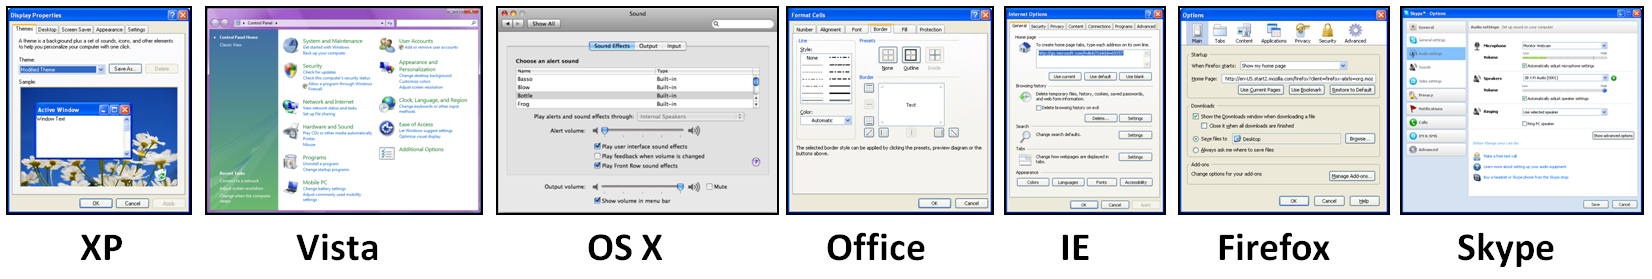
\includegraphics[width=2\columnwidth]{figure/query_examples.png}
\caption{Examples of query images used in screenshot matching
experiments.}
\label{fig:query_examples}
\end{figure*}


\subsection{Compare to keyword search}

In this experiment, we compared the proposed multi-modal search engine
to two keyword search baselines. The first baseline is a commerical
web search engine.  The second baseline is a commerical image search
engine. We were interested in whether users would judge the search
results returned by these three systems differently in terms of
perceived relevancy. We recruited workers from Amazon Mechanical Turk
to perform relevancy judgement.

The comparison is based on 20 query instances (10 XP and 10 Mac
programs). Each query instance was submitted to each of the three
systems. For the two keyword search baselines, we used the words in
the title bar of each program and the name of the operating system as
search terms, for example, mac system preferences. For our system, we
used only the screenshot of the program as the search term. We
collected the top four articles returned by each system and merged
them into a single list of 12. As validation, we added 3 irrelevant
articles and 1 duplicate article to the list. Irrelevant articles were
generated by sampling from the top results returned by the image
search baseline using only one of the search terms, for example, using
the word preferences as the search term for mac system
preferences. Thus, in each assignment, a worker was shown a list of 16
articles and asked to rate the relevancy on a 5-point scale. The list
was randomly shuffled to remove any bias due to ordering.  We only
accepted the ratings given by workers who rated the validation
articles accurately, which was checked by (1) whether irrelevant
articles were rated as irrelevant and (2) whether duplicate articles
were rated consistently. The presence of validation checks
ensure that the optiaml strategies for the workers is to
provide answer in an honest manner.

In total, we obtained X unique ratings from Y workers. The 
approval rate was Z. Table X summarizes our findings. 

\subsection{Bilingual search}

In this experment, we examined the ability of our system to search
across language boundaries. We took screenshots of 15 representative
programs on Mac in five languages (Spanish, French, German,
Chinese, and Korean) and obtained a total of 75 test
images.  We submitted these images to our 
system and retrieved the top 10 matched screenshots. We recorded
the number of correct matches. Table X summarizes
our findings.

\begin{figure*}
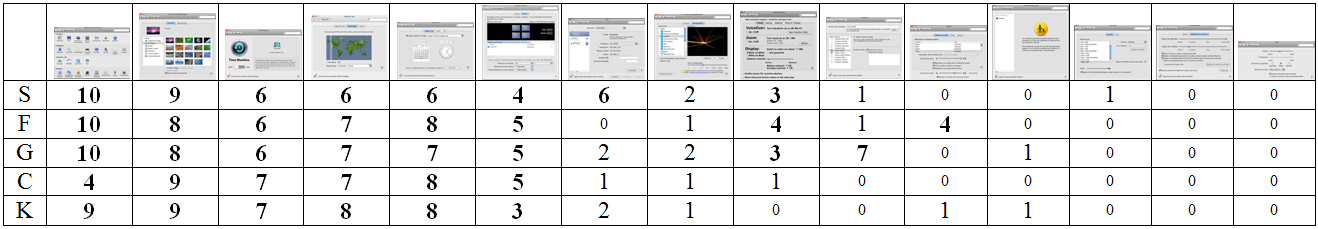
\includegraphics[width=2\columnwidth]{figure/bilingual_search.png}
\caption{Number of correct top 10 matches for 15 programs in five non-English
languages: Spanish (S), French (F), German (G), Chinese (C) and Korean (K).}
\end{figure*}


\section{Discussion}

Keywords can serve two purposes. First, they can specify the
content users wish to see on the returned pages. Second, they can
describe the screenshot to improve the performance of visual
matching. Since the screenshot matching can be done very
accurately, we expect users will very quickly realize that it is
not necessary to repeat the text embedded in the screenshot, since
the visual search will take care of it.


\section{Summary}

\bibliographystyle{plain}
\bibliography{www2010}
\balancecolumns % GM July 2000
% That's all folks!
\end{document}
